\section{Introduction}
\begin{figure}[H]
	\center
	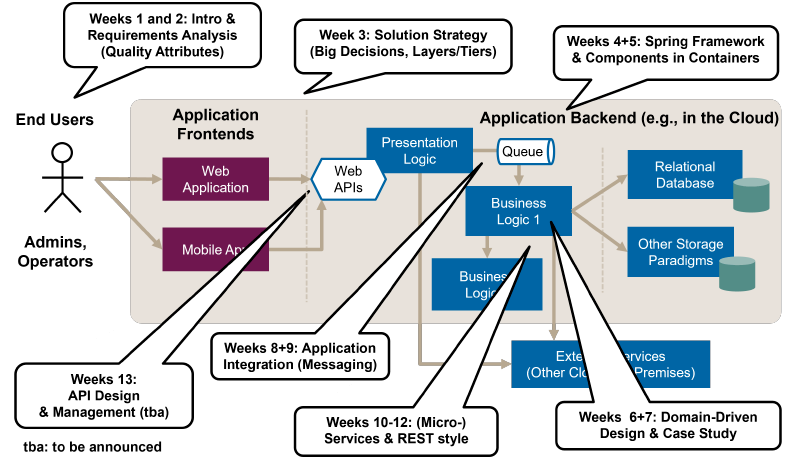
\includegraphics[width=0.75\textwidth]{moduleoverview}
	\caption{Module Overview}
	\label{fig:moduleoverview}
\end{figure}
There is a difference between Information Technology/Software Architecture and Application Architecture. Software Architecture includes the operation and security of the running software, on the other hand Application Architecture does mainly cover the static architecture.

What is Software Architecture?
\begin{description}
	\item [Bass, Clemens, Kazman, 1998] The \textbf{structure} or structures of the system, which comprise software\textbf{elements}, the externally visible \textbf{properties} of those elements, and the \textbf{relationship} among them.
	\item [Jansen, Bosch, 2005] A software systems architecture is a set of \textbf{principle design decision} made about the system.
	\item [ISO/IEC/IEEE 42010, 2011] The fundamental organization of a system is embodied in its \textbf{components}, their \textbf{relationships} to each other, and to the environment, and the \textbf{principles} guiding its designs and evolution.
\end{description}

\textbf{What is Architectural significant?}
\begin{itemize}
	\item Number of Users
	\item Availability
	\item Lifetime
	\item Extendability
	\item Regulations
	\item Laws
	\item Safety and Security
\end{itemize}

\subsection{High-Level Example}
Architecture is everywhere in software engineering. An example can be the process automation and supervision in  the production industry. All layers in the automation pyramid, from sensors and actuators to Distributed Control Systems (DCS) are part of it. An example shows Figure \ref{fig:automationpyramid} of ABB.

\begin{figure}[H]
	\center
	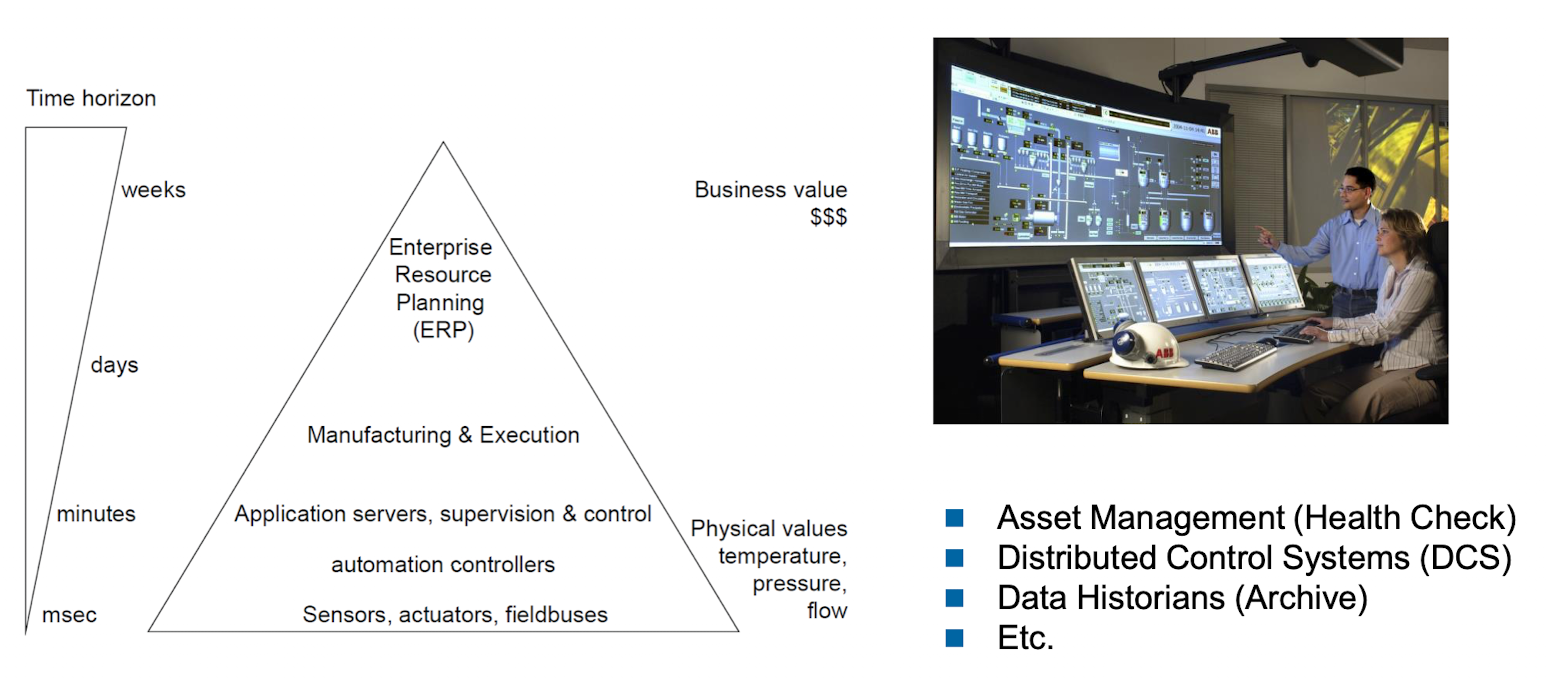
\includegraphics[width=0.75\textwidth]{highlevelarchitecture}
	\caption{Automation Pyramid of ABB}
	\label{fig:automationpyramid}
\end{figure}

\subsection{Architectural Significance Requirements (ASRs)}
Architecturally significant requirements are those requirements that have a measurable effect on a computer system’s architecture. ASRs help the developer/architect to prioritize technical issues or requirements quickly so that architecturally significant issues are addressed at their most responsible moment and we do not have to revise decisions and designs unnecessarily later.

The time budget per issue is one to two minutes at most, as it is not unusual to be confronted with 10 to 100 issues per day — thanks to email and auto-notifications in tools such as Kanban boards, issue trackers, and source code management systems.

\paragraph{Architecturally Significant Requirements} \hfill \\
The following points enable a developer to check if a requirement is architecturally significant, therefore make an ASR test. The points six and seven are very subjective and often not considered as must have for a story to be architectural significant.

\begin{enumerate}
	\item The requirement is directly associated with high \textbf{business value} or \textbf{business risk}.
	\item The requirement is a \textbf{concern} of a particularly \textbf{important stakeholder} (for instance, the project sponsor or an external compliance auditor).
	\item The requirement has runtime \textbf{Quality-of-Service (QoS)} characteristics (e.g., performance needs) that deviate from those already satisfied by the evolving architecture substantially.
	\item The requirement causes new or deals with one or more existing \textbf{external dependencies} that have unpredictable, unreliable and/or uncontrollable behaviour.
	\item The requirement has a \textbf{cross-cutting nature} and therefore affects multiple parts of the system and their interactions; it may even have \textbf{system-wide impact}.
	\item The requirement has a \textbf{first-of-a-kind} character: e.g., the team has never built a component that satisfies this particular requirement.
	\item The requirement has been \textbf{troublesome} and caused critical situations, budget overruns or client dissatisfaction \textbf{in a previous project} in a similar context.
\end{enumerate}

\paragraph{Example ASR Test} \hfill \\
The following paragraph gives an example analysis of requirements regrading their architectural significance. Please make sure to always justify the answer in order to make them understandable.

\begin{table}[H]
	\resizebox{\textwidth}{!}{%
		\begin{tabular}{|l|l|l|l|}
			\hline
			\textbf{Requirement}                                                     &
			\textbf{Score}                                                           &
			\textbf{Mapping}                                                         &
			\textbf{Explanation}                                                                                                                                                                                                                                                                                                                                                    \\ \hline
			Autoscaling for Spinnaker microservices running on Kubernetes            &
			High (H)                                                                 &
			\begin{tabular}[c]{@{}l@{}}RC-2, RC-3, RC-4\\ Possibly RC-7\end{tabular} &
			\begin{tabular}[c]{@{}l@{}}Auto scaling may have an impact on\\ the billing, so external stakeholder\\ affected (cloud provider); scalability is\\ a key quality attribute; dependency on\\ 3rd party software; autonomous\\ system behavior has been reported to\\ be hard to test and maintain due to\\ number of external stimuli and time\\ dependency\end{tabular} \\ \hline
		\end{tabular}%
	}
	\caption{Sample Requirement Analysis for Architectural Significance}
\end{table}

\subsection{SMART Non-Functional Requirements}
The SMART criteria are frequently used in project and people management, but they can also be applied to Non-Functional Requirement (NFR) engineering. Most of the time only \textit{S} and \textit{M} are used in NFR engineering.

\begin{description}
	\item [\textit{S}pecific] Which feature or part of the system should satisfy the requirement. (scoping the requirement)
	\item [\textit{M}easurable] How can testers and other stakeholders fond out whether the requirement is met (or not)? Is the requirement quantified. (monitoring the requirement)
	\item [\textit{A}agreed Upon] The goal must be realistic and achievable and a consent in the team.
	\item [\textit{R}elevant/Realistic] One must be aware of why one wants to achieve it.
	\item [\textit{T}ime-Bound] With a clearly defined timeline, including a starting date and a target date.
\end{description}

\paragraph{Architectural Significance of Design Elements} \hfill \\
In addition to the ASRs there is also the need to to specify is a structural design element (e.g. component, connector, class, OOP method) is considered architecturally significance.

\begin{enumerate}
	\item The element is associated with some \textbf{critical functionality} of the system / e.g. money transfer
	\item The element is associated with a \textbf{critical quality} on the solution / e.g. performance of distributed communication
	\item The element is associated with a \textbf{critical constraint} of the solution / e.g. access to an external system
	\item The element incurs a particular  \textbf{technical risk} / e.g. access to a never-before-tried capability
	\item The element presents a \textbf{particular architectural change} / e.g. high transaction volume
\end{enumerate}

A table is the obvious format for the resulting seven-criteria ASR test as displayed in the Figure \ref{fig:asrtest}.

\begin{figure}[H]
	\center
	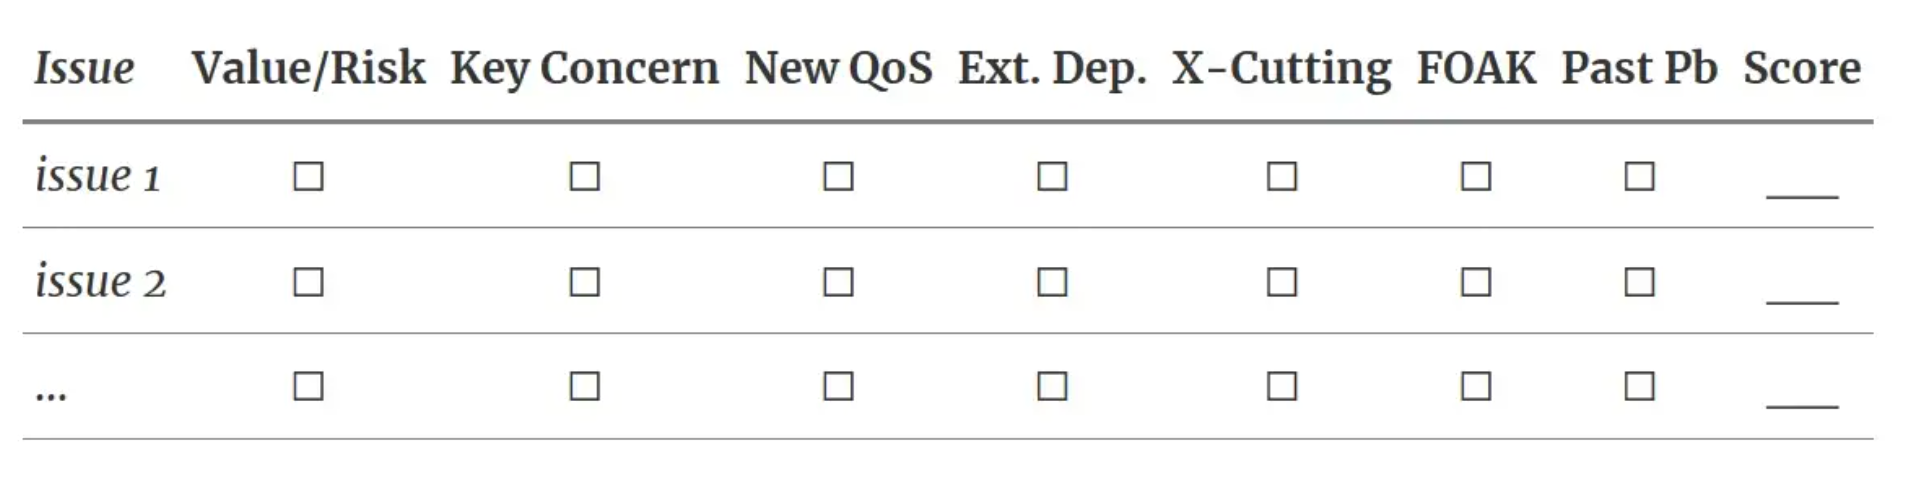
\includegraphics[width=0.75\textwidth]{asrtest}
	\caption{A Scoring/Assessment Tempalte Table}
	\label{fig:asrtest}
\end{figure}

\subsection{FURPS+}
The FURPS+ acronym, devised by Robert Grady of HP, provides a way to define requirements by non-functional stories, and also provides a good way to categorize such needs. The breakdown here suggests some representative questions around potential needs.

\begin{description}
	\item [F]unctionality: represents the main product features that are familiar within the business domain of the solution being developed. The functional requirements can also be very technically oriented.
	\item [U]sability: includes looking at, capturing, and stating requirements based around user interface issues — things such as accessibility, interface aesthetics, and consistency within the user interface.
	\item [R]eliability: includes aspects such as availability, accuracy, and recoverability — for example, computations, or recoverability of the system from shut-down failure.
	\item [P]erformance: involves things such as throughput of information through the system, system response time (which also relates to usability), recovery time, and start-up time.
	\item [S]upportability: we tend to include a section called supportability, where we specify a number of other requirements such as testability, adaptability, maintainability, compatibility, configurability, installability, scalability, localizability, and so on.
	\item [+] allows us to specify constraints, including design, implementation, interface, and physical constraints.
\end{description}

\paragraph{Example FURPS+ Requirements}
\begin{description}
	\item [F] As a meeting organiser, i would like to propose some time slots so that invitees can indicate their availability, which eases my decisions making and further planning.
	\item [U] All information should be displayed on one page/screen; adding a time slot should be a single step that can be completed in a few seconds.
	\item [R] The calendar service should be highly available during office hours (8am to 5pm); it should not crash when invalid data is entered
	\item [P] Time slot additions should be confirmed and displayed correctly within two seconds; the overview page should load within one second.
	\item [S] Severity 1 bugs are fixed within 48 business hours, severity 2 issues within one calendar week.
\end{description}
